% datasets.tex

\marginnote{beginning of datasets.tex}

\begin{figure}
  \centering

\includegraphics[width=120mm]{images/articulator.png}
\caption{Synthetic examples of a shape with an articulation point.}
\label{fig-articulator}
\end{figure}

\begin{figure}
  \centering
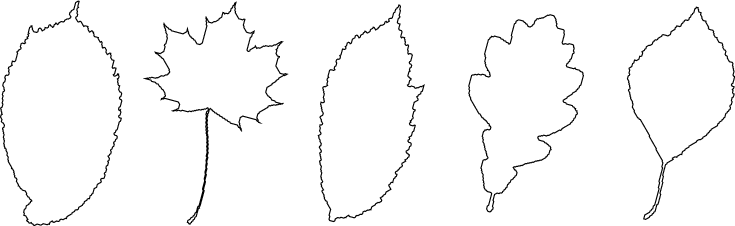
\includegraphics[width=120mm]{images/leaves.png}
\caption{The Swedish leaves dataset.}
\label{fig-leaves}
\end{figure}

\begin{figure}
  \centering
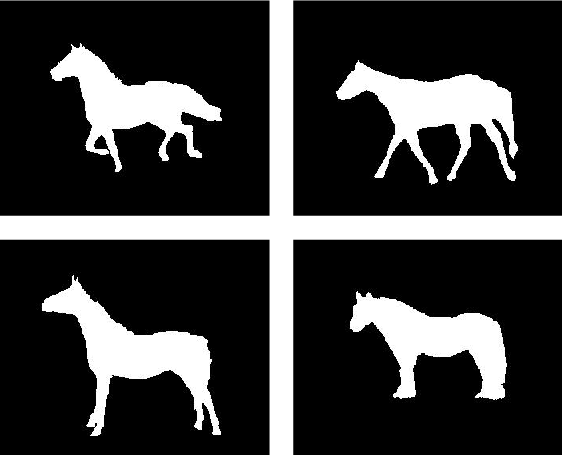
\includegraphics[width=120mm]{images/horse.png}
\caption{The Weizmann horse dataset.}
\label{fig-horse}
\end{figure}

\begin{figure}
  \centering
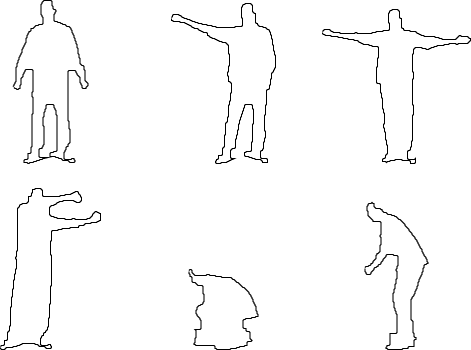
\includegraphics[width=120mm]{images/romer.png}
\caption{The Romer dataset.}
\label{fig-romer}
\end{figure}

\marginnote{end of datasets.tex}
